\chapter{Theoretische Grundlagen}
\label{chap:two}
\section{Bibliothek und Statistik}
\label{chap:two_one}

Erhebung von qualitativen und quantitativen Daten
Bsp.:

Konzentration auf quantitative Daten wie ...

Bestandsmanagement\\
Nutzungsanalyse\\
Counter-Statistiken \& Standards
Bestandsanalyse -und Evaluierung\\

Warum ist Messbarkeit von bibliothekarischen Daten wichtig?\\
Was können statistische Daten in Bibliotheken aussagen?\\
Welchen Impact für Budgetplanung können statistische Daten haben?\\

Counter5Statistiken
\section{Datenvisualisierung und Datenvisualisierungstechniken}
Was ist unter Datenvisualisierung zu verstehen?\\
Warum Datenvisualisierung wichtig ist?\\
Welche Datenvisualisierungen gibt es?\\
Was erzählen Datenvisualisierungen mehr als Zahlenkolonnen?\\
Wo kommen Daternvisualisierungen zum Einsatz?\\
Was ist unter Datenvisualisierungstechniken zu verstehen?\\
Wo kommen Datenvisualisierungstechniken zum Einsatz?


\begin{figure}[ht]
    \centering
        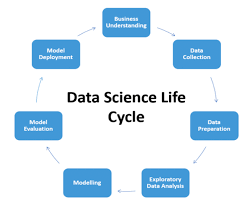
\includegraphics[width=8cm]{ds_cycle}
        \caption{Data Science Cycle}
        \label{fig:data science}
\end{figure}




\section{Business-Intelligence-Systeme}

Was sind Business-Intelligence-Löungen?\\
Wo kommen Buisiness-Intelligence-Lösungen zum Einsatz zum Einsatz?
